%%%%%%%%%%%%%%%%%%%%%%%%%%%%%%%%%%%%%%%%%%%%%%%%%%%%%%%%%%%%%%%%%%%%%%%%%%%%%%%
%                       CARREGA DE LA CLASSE DE DOCUMENT                      %
%                                                                             %
% Les opcions admissibles son:                                                %
%      12pt / 11pt            (cos dels tipus de lletra; no feu servir 10pt)  %
%                                                                             %
% catalan/spanish/english     (llengua principal del treball)                 %
%                                                                             % 
% french/italian/german...    (si necessiteu fer servir alguna altra llengua) %
%                                                                             %
% listoffigures               (El document inclou un Index de figures)        %
% listoftables                (El document inclou un Index de taules)         %
% listofquadres               (El document inclou un Index de quadres)        %
% listofalgorithms            (El document inclou un Index d'algorismes)      %
%                                                                             %
%%%%%%%%%%%%%%%%%%%%%%%%%%%%%%%%%%%%%%%%%%%%%%%%%%%%%%%%%%%%%%%%%%%%%%%%%%%%%%%

\documentclass[11pt,spanish,listoffigures,listoftables]{tfgetsinf}

%%%%%%%%%%%%%%%%%%%%%%%%%%%%%%%%%%%%%%%%%%%%%%%%%%%%%%%%%%%%%%%%%%%%%%%%%%%%%%%
%                     CODIFICACIO DEL FITXER FONT                             %
%                                                                             %
%    windows fa servir normalment 'ansinew'                                   %
%    amb linux es possible que siga 'latin1' o 'latin9'                       %
%    Pero el mes recomanable es fer servir utf8 (unicode 8)                   %
%                                          (si el vostre editor ho permet)    % 
%%%%%%%%%%%%%%%%%%%%%%%%%%%%%%%%%%%%%%%%%%%%%%%%%%%%%%%%%%%%%%%%%%%%%%%%%%%%%%%

\usepackage[utf8]{inputenc} 

\usepackage{natbib}
\bibliographystyle{plain}
\graphicspath{ {Imagenes/} }

%%%%%%%%%%%%%%%%%%%%%%%%%%%%%%%%%%%%%%%%%%%%%%%%%%%%%%%%%%%%%%%%%%%%%%%%%%%%%%%
%                        ALTRES PAQUETS I DEFINICIONS                         %
%                                                                             %
% Carregueu aci els paquets que necessiteu i declareu les comandes i entorns  %
%                                          (aquesta seccio pot ser buida)     %
%%%%%%%%%%%%%%%%%%%%%%%%%%%%%%%%%%%%%%%%%%%%%%%%%%%%%%%%%%%%%%%%%%%%%%%%%%%%%%%



%%%%%%%%%%%%%%%%%%%%%%%%%%%%%%%%%%%%%%%%%%%%%%%%%%%%%%%%%%%%%%%%%%%%%%%%%%%%%%%
%                        DADES DEL TREBALL                                    %
%                                                                             %
% titol, alumne, tutor i curs academic                                        %
%%%%%%%%%%%%%%%%%%%%%%%%%%%%%%%%%%%%%%%%%%%%%%%%%%%%%%%%%%%%%%%%%%%%%%%%%%%%%%%

\title{ Desarrollo de software basado en microservicios: un caso de estudio para evaluar sus ventajas e inconvenientes }
\author{Víctor Alberto Iranzo Jiménez}
\tutor{Patricio Orlando Letelier Torres}
\curs{2017-2018}

%%%%%%%%%%%%%%%%%%%%%%%%%%%%%%%%%%%%%%%%%%%%%%%%%%%%%%%%%%%%%%%%%%%%%%%%%%%%%%%
%                     PARAULES CLAU/PALABRAS CLAVE/KEY WORDS                  %
%                                                                             %
% Independentment de la llengua del treball, s'hi han d'incloure              %
% les paraules clau i el resum en els tres idiomes                            %
%%%%%%%%%%%%%%%%%%%%%%%%%%%%%%%%%%%%%%%%%%%%%%%%%%%%%%%%%%%%%%%%%%%%%%%%%%%%%%%

\keywords{Microservices, Arquitecturas de software, ?????????????????} % Paraules clau 
         {Microservicios, Arquitecturas de software, ???????????????}              % Palabras clave
         {Microservices, Software Architecture, ?????????????}        % Key words

%%%%%%%%%%%%%%%%%%%%%%%%%%%%%%%%%%%%%%%%%%%%%%%%%%%%%%%%%%%%%%%%%%%%%%%%%%%%%%%
%                              INICI DEL DOCUMENT                             %
%%%%%%%%%%%%%%%%%%%%%%%%%%%%%%%%%%%%%%%%%%%%%%%%%%%%%%%%%%%%%%%%%%%%%%%%%%%%%%%

\begin{document}

%%%%%%%%%%%%%%%%%%%%%%%%%%%%%%%%%%%%%%%%%%%%%%%%%%%%%%%%%%%%%%%%%%%%%%%%%%%%%%%
%              RESUMS DEL TFG EN VALENCIA, CASTELLA I ANGLES                  %
%%%%%%%%%%%%%%%%%%%%%%%%%%%%%%%%%%%%%%%%%%%%%%%%%%%%%%%%%%%%%%%%%%%%%%%%%%%%%%%

\begin{abstract}
????
\end{abstract}
\begin{abstract}[spanish]
????
\end{abstract}
\begin{abstract}[english]
????
\end{abstract}

%%%%%%%%%%%%%%%%%%%%%%%%%%%%%%%%%%%%%%%%%%%%%%%%%%%%%%%%%%%%%%%%%%%%%%%%%%%%%%%
%                              CONTINGUT DEL TREBALL                          %
%%%%%%%%%%%%%%%%%%%%%%%%%%%%%%%%%%%%%%%%%%%%%%%%%%%%%%%%%%%%%%%%%%%%%%%%%%%%%%%

\mainmatter

%%%%%%%%%%%%%%%%%%%%%%%%%%%%%%%%%%%%%%%%%%%%%%%%%%%%%%%%%%%%%%%%%%%%%%%%%%%%%%%
%                                  INTRODUCCIO                                %
%%%%%%%%%%%%%%%%%%%%%%%%%%%%%%%%%%%%%%%%%%%%%%%%%%%%%%%%%%%%%%%%%%%%%%%%%%%%%%%

\chapter{Introducci\'on}

\section{Motivaci\'on}

% Referencia a The Clean Architecture.
En la actualidad, no es necesario un alto grado de conocimientos en ingeniería del software para desarrollar una aplicación o sistema. Personas que no tienen estudios relacionados con la informática pueden producir código que, sin ser limpio y elegante, funciona. Desarrollar sistemas de calidad requiere de grandes conocimientos, pero minimiza los costes y aumenta la productividad de una organización. Se debe poner el foco en emplear una arquitectura de software que se adapte a nuestras necesidades. De lo contrario, el futuro mantenimiento será más costoso y repercutirá en la confianza de los clientes y en la moral del equipo. \cite{Martin2017}

% TODO: Demasiados términos que se deben explicar.
Las arquitecturas basadas en microservicios son una tendencia actual que emerge asociada a conceptos clave como la integración continua, el desarrollo centrado en el dominio del problema o el despliegue en contenedores. En estas arquitecturas diferentes funcionalidades se encapsulan en servicios pequeños y autónomos que cooperan entre ellos. En términos de diseño, principios como el de Responsabilidad Única son más fáciles de conseguir y los desafíos de organización del código pueden abordarse de formas más diversas por la baja granularidad de la arquitectura. 

\section{Objetivos}

El objetivo de este proyecto es validar con un caso de estudio las ventajas e inconvenientes de una arquitectura basada en microservicios frente a una arquitectura monolítica. Concretamente,los objetivos específicos son:

\begin{itemize}

\item Desarrollar una misma aplicación para la venta de productos y la gestión de pedidos siguiendo dos arquitecturas diferentes: una basada en microservicios y otra monolítica.

\item Comparar el proceso de desarrollo de ambos sistemas a lo largo del ciclo de vida del software.

\item Evaluar cómo se pueden llevar a cabo diferentes modificaciones durante el mantenimiento de ambas aplicaciones una vez se ha finalizado su implementación.

\item Verificar que una arquitectura basada en microservicios facilita alcanzar los requisitos no funcionales de disponibilidad y tolerancia a fallos frente a una arquitectura monolítica.

\end{itemize}

\section{Estructura de la memoria}

\chapter{Estado del arte}

\section{¿Qué son los microservicios?}

Según Newman, los microservicios son servicios pequeños y autónomos que trabajan conjuntamente. \cite{Newman2015a} Podemos desglosar esta definición así:

\begin{itemize}

\item Un \textbf{servicio} es un conjunto de funcionalidades que se expone a los clientes para que las empleen con diferentes propósitos. \cite{Wikipedia} La programación orientada a servicios es un paradigma que se aplica en las arquitecturas orientadas a servicios (SOA). El objetivo principal de SOA es desarrollar servicios que aporten valor al negocio y se adapten a los cambios en las necesidades de los clientes, de forma ágil y con el menor coste posible. Las arquitecturas orientadas a servicios no están asociadas a ninguna tecnología específica. En líneas generales, dividen un sistema en componentes que cambian por el mismo motivo y promueven la flexibilidad y los servicios compartidos frente a implementaciones específicas y óptimas. Son muchos los beneficios de estas arquitecturas, sin embargo existe una falta de consenso sobre cómo debe llevarse a cabo este tipo de arquitecturas en aspectos como los protocolos de comunicación a emplear o la granularidad de los servicios. \cite{Arsanjani2009a} Los microservicios pueden entenderse como una aproximación específica de las arquitecturas SOA.

\item Diseñar microservicios con el menor \textbf{tamaño} posible no debe ser el foco principal. En todo momento han de cumplirse los principios de cohesión y coherencia: el código relacionado debe agruparse conjuntamente porque será modificado por el mismo motivo. Una regla que puede ser aplicada según el autor Jon Eaves es establecer un tamaño para un microservicio tal que pueda ser completamente reescrito en 2 semanas.

\item  Los servicios han de ser lo menos acoplados posibles para garantizar la \textbf{autonomía} de cada uno. Cada microservicio es una entidad separada: cambian de forma independiente al resto y al hacerlo sus consumidores no necesiten ser modificados, a menos que se modifique el contrato entre ambas partes. Para lograrlo, lo más habitual es que cada servicio exponga una interfaz (API) y todas las comunicaciones se realicen mediante llamadas a través de la red.

\end{itemize}

Otra definición interesante es la que aportan Lewis y Fowler. Según ellos, los microservicios son una aproximación para desarrollar una aplicación compuesta por pequeños servicios, cada uno ejecutándose en su propio proceso y comunicando a través de mecanismos ligeros. Estos servicios se construyen alrededor de las capacidades de negocio y se despliegan de forma independiente. \cite{Lewis2014} Cada funcionalidad se encapsula en un servicio que puede escalar de forma diferente de acuerdo a sus necesidades, a diferencia de las aplicaciones monolíticas donde se debe replicar el monolito al completo.

\begin{figure}[h]
\centering
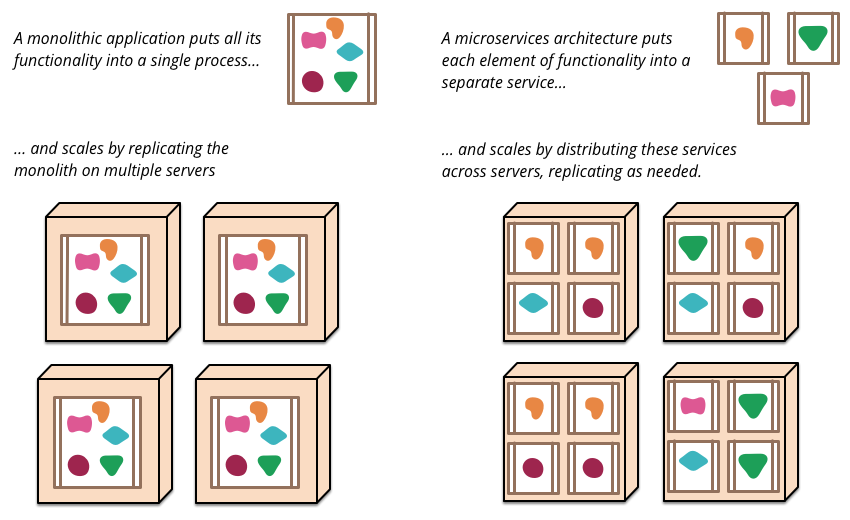
\includegraphics[scale=0.4]{microservices_escaling}
\caption{Los microservicios escalan de acuerdo a su carga de trabajo para asegurar la disponibilidad de la funcionalidad que ofrecen. \cite{Lewis2014}}
\end{figure}

\section{Los microservicios en la fase de requisitos}

La fase de requisitos del software es aquella en la que se elicitan, analizan, documentan, validan y mantienen los requisitos del sistema. Los requisitos del software expresan las necesidades y restricciones asociadas a un sistema. \cite{Fernandes2016} El artefacto principal que se produce en esta fase es el documento con la especificación de requisitos software (ERS). Una vez validado dicho documento por los stakeholders se puede iniciar la fase de diseño la solución. Esto no significa el final de esta fase del proceso: la gestión de los requisitos continúa durante el resto del desarrollo del producto.

\subsection{Requisitos funcionales y no funcionales}

Los requisitos se pueden clasificar en funcionales y no funcionales. Los \textbf{requisitos funcionales} (RF) describen la funcionalidad que los usuarios esperan del sistema. Los \textbf{requisitos no funcionales} (RNF) son restricciones impuestas sobre el sistema a desarrollar, estableciendo por ejemplo como de rápido o fiable ha de ser. Mientras que los primeros no incluyen ninguna mención relacionada con la tecnología que emplea el sistema, los segundos sí pueden establecer restricciones de este tipo. Por ejemplo, un requisito no funcional puede consistir en desarrollar una aplicación en un lenguaje de programación específico o hacer que esté disponible para diferentes sistemas operativos móviles. Por este motivo, los requisitos deben ser tenidos en cuenta a lo largo de todo el desarrollo del sistema.

Los requisitos funcionales y no funcionales son ortogonales en el sentido de que diferentes diseños de software pueden ofrecer la misma funcionalidad (RF) pero con distintos atributos de calidad (RNF). Los arquitectos software están más centrados en los requisitos no funcionales porque estos son los que conducen hacia la elección de una u otra arquitectura. Los requisitos no funcionales pueden influir en los patrones arquitectónicos a seguir, las futuras estrategias de implementación del sistema o la plataforma sobre la que se desplegará el sistema. \cite{Ameller2013}

\begin{figure}[h]
\centering
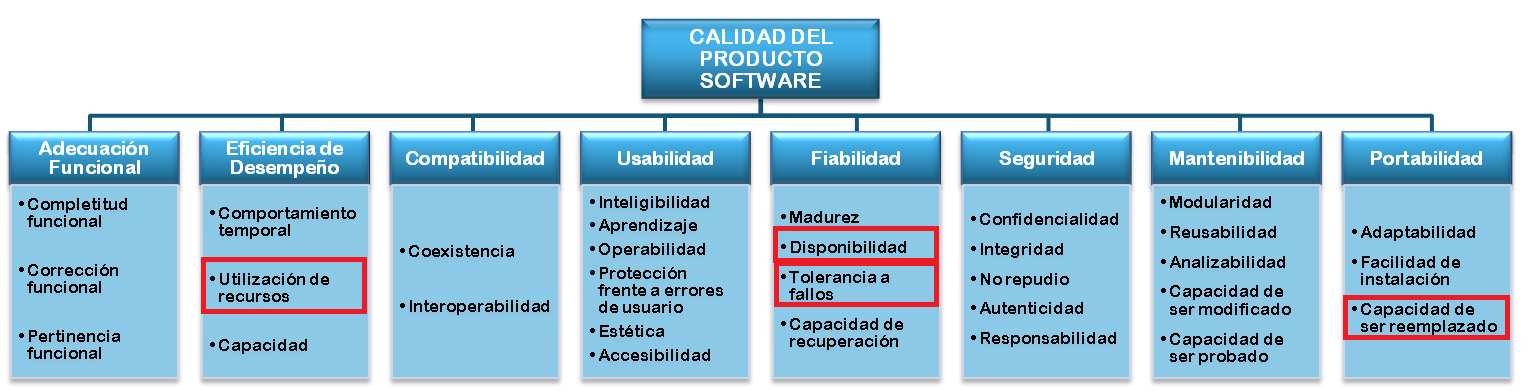
\includegraphics[scale=0.5]{iso25010}
\caption{Características y subcaracterísticas definidas en el modelo de calidad del producto de la ISO/IEC 25010. \cite{Standard2010}}
\end{figure}

Requisitos no funcionales asociados a atributos de calidad como la tolerancia a fallos o la disponibilidad pueden conducir al arquitecto hacia la elección de una arquitectura basada en microservicios:

\begin{itemize}

\item La \textbf{tolerancia a fallos} se define como la capacidad del sistema para operar según lo previsto en presencia de fallos hardware o software. \cite{Standard2010} Cuando se escala un sistema, la probabilidad de fallo es inevitable. Muchas organizaciones invierten mucho esfuerzo en evitar que un fallo se produzca, pero muy poco en mecanismos para recuperar el sistema una vez se ha producido. Un sistema que por culpa de un servicio caído deja de funcionar es menos resilente que un sistema que puede continuar ofreciendo el resto de sus funcionalidades.

\item La \textbf{disponibilidad} se define en la ISO/IEC 25010 como la capacidad del sistema de estar operativo y accesible para su uso cuando se requiere. \cite{Standard2010} En los sistemas distribuidos existen 3 características sobre las que se debe hacer balance: la consistencia, que establece que vamos a obtener una respuesta correcta de cualquier nodo de un servicio de acuerdo a su especificación, la disponibilidad, que ya hemos definido, y la tolerancia a particiones, que es la habilidad de gestionar situaciones en las que la comunicación entre las partes de un sistema se interrumpe. El teorema de CAP (debe sus siglas a las características en inglés Consistency, Availability y Partition Tolerance) establece que en caso de fallo, solo dos de las tres características pueden prevalecer. \cite{Gilbert2012}

\end{itemize}

\subsection{El teorema de CAP}

Pongamos un ejemplo en el que un microservicio está replicado y se produce un fallo por el cual la comunicación entre las replicas se interrumpe y los cambios en una replica no se pueden propagar al resto. Los \textbf{sistemas AP} son los sistemas que surgen fruto de sacrificar la consistencia cuando un fallo se produce, mientras que en los \textbf{sistemas CP} se pierde la disponibilidad. En el primer tipo, las replicas continuarían operativas, pero como los datos entre las replicas no se sincronizan se pueden obtener datos incorrectos al hacer una consulta. Cuando la comunicación se restablece, los cambios entre las replicas se sincronizarán. En los sistemas CP, para mantener la consistencia entre las replicas se tiene que rechazar cualquier petición, con lo que el servicio deja de estar disponible.

Los sistemas AP escalan más fácilmente y son más sencillos de construir, pero nos obligan a una consistencia eventual de los datos. Los segundos son los únicos que nos aseguran una consistencia fuerte, pero son más difíciles de construir. A la hora de optar por una solución u otra se debe tener en cuenta la especificación de requisitos, donde se debe detallar de forma específica y cuantitativa cuánto tiempo puede nuestro servicio estar inoperativo o con un dato obsoleto. Si en las fases siguientes se opta por una arquitectura basada en microservicios, no será necesario implementar el sistema completo de una u otra forma. Cada microservicio tendrá necesidades diferentes y podrá seguir la aproximación que mejor le convenga. \cite{Newman2015a}

\section{Los microservicios en la fase de diseño}

En la fase de diseño se definen la arquitectura, componentes e interfaces del sistema. La especificación de requisitos es analizada para producir una descripción de la estructura interna del sistema, con el suficiente nivel de detalle para que sirva como base en su construcción. En esta fase se plantean diferentes diseños como alternativas de las que se debe hacer balance. Los modelos que se generan se emplearán para validar que se cumplen los requisitos establecidos y para planificar la fase de implementación. \cite{Bourque2014}

\subsection{Librerías versus servicios}

Un componente es una unidad de software que se puede reemplazar y actualizar de forma independiente. Las librerías son componentes que están ligados a un programa y son invocadas a través de llamadas a funciones. En cambio, los servicios son componentes que se ejecutan como procesos externos y con los que se puede comunicar a través de mecanismos como llamadas a procedimientos remotos (RPC) o peticiones HTTP. \cite{Lewis2014}

Uno de los motivos por los que se recomienda emplear servicios frente a librerías es que los servicios se pueden desplegar de forma independiente. Solo algunos cambios en la interfaz o contrato del servicio requerirán un cambio en sus consumidores. Sin embargo, las llamadas remotas son más costosas que las invocaciones dentro del mismo proceso, por lo que la interfaz del servicio debe definirse de tal forma que sus consumidores no tengan que comunicarse con él continuamente.

\subsection{La tarea del arquitecto}

El software ha de ser diseñado para ser flexible, adaptarse y evolucionar en función de los requisitos de los usuarios. En lugar de centrarse en diseñar un producto final perfecto, el arquitecto debe crear un entorno donde el sistema correcto pueda emerger creciendo progresivamente a medida que se descubren nuevos requisitos. Gracias a su modularidad, los microservicios son el entorno perfecto para que esto ocurra.

El arquitecto de software debe preocuparse más por como interaccionan los servicios entre ellos y no tanto en lo que ocurre dentro de sus límites. En organizaciones grandes, cada microservicio puede estar desarrollado por un equipo distinto y es el arquitecto quien debe hacer de puente entre ellos. \cite{Newman2015a}

Una de las ventajas de las arquitecturas basadas en microservicios es la heterogeneidad tecnológica: cada servicio puede ser desarrollado empleando una pila tecnológica distinta. No obstante, dejar plena libertad a cada equipo para elegir la tecnología del servicio que va a desarrollar puede traer problemas a la hora de integrarlo con el resto del sistema. El uso de contratos o establecer normas en aspectos clave como el protocolo de comunicación entre los servicios facilitará su consumo. Las decisiones de diseño de un servicio en particular pueden recaer en el equipo responsable. En este caso, el arquitecto solo juega un papel de supervisor y asesor para evitar que se pierda la imagen del sistema completo.

\section{Los microservicios en la fase de implementación}

\section{Los microservicios en la fase de pruebas}

\section{Los microservicios en la fase de despliegue}

\section{Los microservicios en la fase de mantenimiento}

\section{Ventajas del desarrollo de software basado en microservicios}

\section{Inconvenientes del desarrollo de software basado en microservicios}

%%%%%%%%%%%%%%%%%%%%%%%%%%%%%%%%%%%%%%%%%%%%%%%%%%%%%%%%%%%%%%%%%%%%%%%%%%%%%%%
%                                 CONCLUSIONS                                 %
%%%%%%%%%%%%%%%%%%%%%%%%%%%%%%%%%%%%%%%%%%%%%%%%%%%%%%%%%%%%%%%%%%%%%%%%%%%%%%%

\chapter{Conclusiones}

????? ????????????? ????????????? ????????????? ????????????? ????????????? 

%%%%%%%%%%%%%%%%%%%%%%%%%%%%%%%%%%%%%%%%%%%%%%%%%%%%%%%%%%%%%%%%%%%%%%%%%%%%%%%
%                                BIBLIOGRAFIA                                 %
%%%%%%%%%%%%%%%%%%%%%%%%%%%%%%%%%%%%%%%%%%%%%%%%%%%%%%%%%%%%%%%%%%%%%%%%%%%%%%%

\bibliography{Bibliografia/library}



%%%%%%%%%%%%%%%%%%%%%%%%%%%%%%%%%%%%%%%%%%%%%%%%%%%%%%%%%%%%%%%%%%%%%%%%%%%%%%%
%                           APÈNDIXS  (Si n'hi ha!)                           %
%%%%%%%%%%%%%%%%%%%%%%%%%%%%%%%%%%%%%%%%%%%%%%%%%%%%%%%%%%%%%%%%%%%%%%%%%%%%%%%

\APPENDIX

%%%%%%%%%%%%%%%%%%%%%%%%%%%%%%%%%%%%%%%%%%%%%%%%%%%%%%%%%%%%%%%%%%%%%%%%%%%%%%%
%                         LA CONFIGURACIO DEL SISTEMA                         %
%%%%%%%%%%%%%%%%%%%%%%%%%%%%%%%%%%%%%%%%%%%%%%%%%%%%%%%%%%%%%%%%%%%%%%%%%%%%%%%

\chapter{Configuración del sistema}

????? ????????????? ????????????? ????????????? ????????????? ?????????????

\section{Fase de inicialización}

????? ????????????? ????????????? ????????????? ????????????? ?????????????

\end{document}
